\documentclass[
  captions=tableheading,
  bibliography=totoc, 
  titepage=firstiscover,
]{scrartcl}

\usepackage{blindtext} %neuer input

\usepackage{longtable} % Tabellen über mehrere Seiten

\usepackage[utf8]{inputenc} %neuer input

\usepackage{scrhack}

\usepackage[aux]{rerunfilecheck} %Warnung falls nochmal kompiliert werden muss

\usepackage{fontspec} %Fonteinstellungen

\recalctypearea{}

\usepackage[main=ngerman]{babel} %deutsche Spracheinstellung

\usepackage{ragged2e} %neuer input

\usepackage{amsmath, nccmath}

\usepackage{amssymb} %viele mathe Symbole

\usepackage{mathtools} %Erweiterungen für amsmath


\DeclarePairedDelimiter{\abs}{\lvert}{\rvert}
\DeclarePairedDelimiter{\norm}{\lVert}{\rVert}

\DeclarePairedDelimiter{\bra}{\langle}{\rvert}
\DeclarePairedDelimiter{\ket}{\lvert}{\rangle}

\DeclarePairedDelimiterX{\braket}[2]{\langle}{\rangle}{
#1 \delimsize| #2
}

\NewDocumentCommand \dif {m}
{
\mathinner{\symup{d} #1}
}


\usepackage[
  math-style=ISO,
  bold-style=ISO,
  sans-style=italic,
  nabla=upright,
  partial=upright,
  warnings-off={
    mathtools-colon,
    mathtools-overbracket,
  },
]{unicode-math}

\setmathfont{Latin Modern Math}
\setmathfont{XITS Math}[range={scr, bfscr}]
\setmathfont{XITS Math}[range={cal, bfcal}, StylisticSet=1]


\usepackage[
  locale=DE,
  separate-uncertainty=true,
  per-mode=reciprocal,
  output-decimal-marker={,},
]{siunitx}

\usepackage[autostyle]{csquotes} %richtige Anführungszeichen

\usepackage{xfrac}

\usepackage{float}

\floatplacement{figure}{htbp}

\floatplacement{table}{htbp}

\usepackage[ %floats innerhalb einer section halten
  section,   %floats innerhalb er section halten
  below,     %unterhalb der Section aber auf der selben Seite ist ok
]{placeins}

\usepackage[
  labelfont=bf,
  font=small,
  width=0.9\textwidth,
]{caption}

\usepackage{subcaption} %subfigure, subtable, subref

\usepackage{graphicx}

\usepackage{grffile}

\usepackage{booktabs}

\usepackage{microtype} %Verbesserungen am Schriftbild

\usepackage[
backend=biber,
]{biblatex}

\addbibresource{../lit.bib}

\usepackage[ %Hyperlinks im Dokument
  german,
  unicode,
  pdfusetitle,
  pdfcreator={},
  pdfproducer={},
]{hyperref}

\usepackage{bookmark}

\usepackage[shortcuts]{extdash}

%\usepackage{warpcol}

\usepackage{physics}
\allowdisplaybreaks

\begin{document}
    \title{Physik IV Übungsblatt 8}
    \author{  
    Tobias Rücker\\
    \texorpdfstring{\href{mailto:tobias.ruecker@tu-dortmund.de}{tobias.ruecker@tu-dortmund.de}
    \and}{,} 
    Paul Störbrock\\
    \texorpdfstring{\href{mailto:paul.stoerbrock@tu-dortmund.de}{paul.stoerbrock@tu-dortmund.de}}{}
    }
\maketitle
\center{\Large Abgabegruppe: \textbf{4H}}
\thispagestyle{empty}

\newpage
\tableofcontents
\thispagestyle{empty}
\newpage

\setcounter{page}{1}

\section{Aufgabe 1}

    \begin{figure}[H]
        \centering
        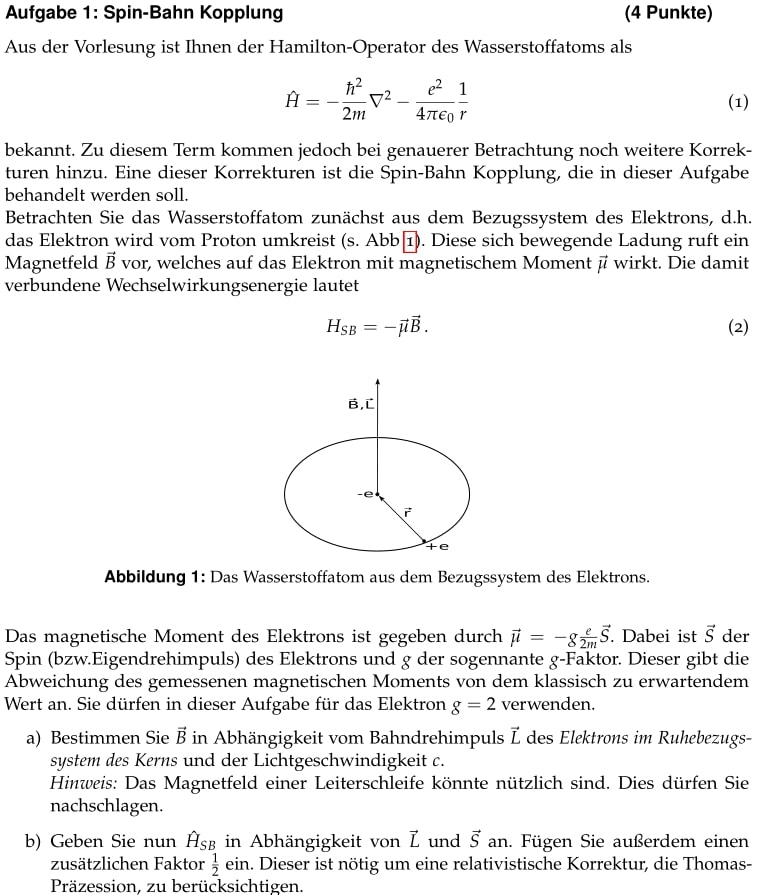
\includegraphics[width=\textwidth]{images/Aufgabe1a.jpg}
        \label{fig:1}
    \end{figure}

    \begin{figure}[H]
        \centering
        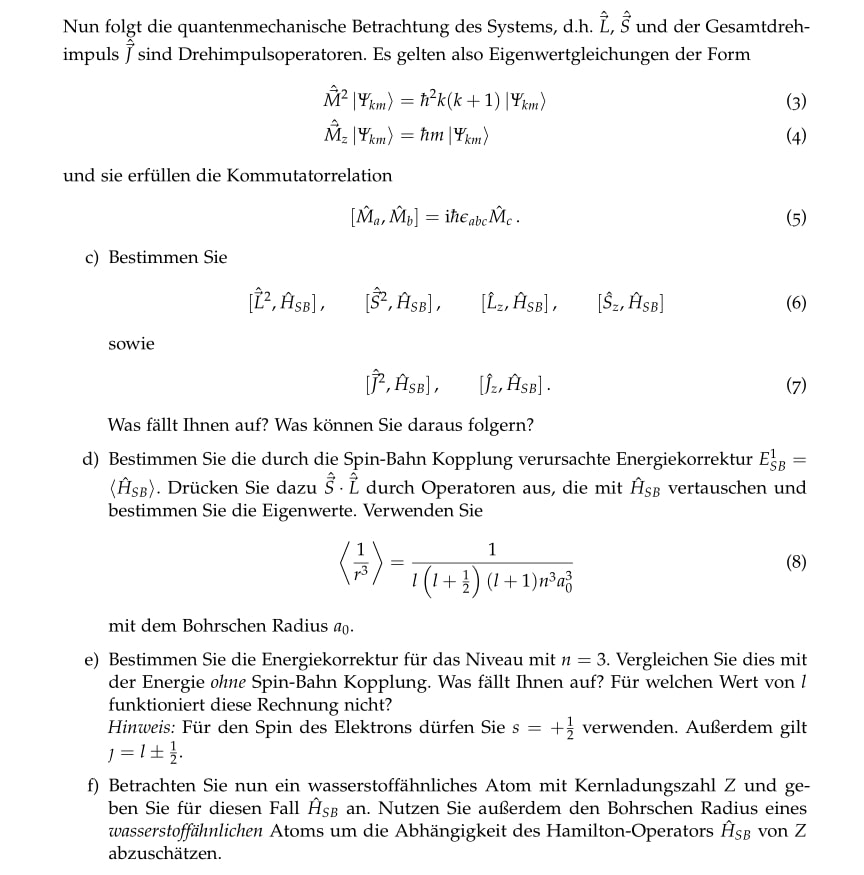
\includegraphics[width=\textwidth]{images/Aufgabe1b.jpg}
        \label{fig:2}
    \end{figure}

    \subsection{a)}
    Das B-Feld einer Leiterschleife lautet:
    \begin{align}
        \vec{B} (z) &= \frac{\mu}{2} \frac{R^2 I}{(R^2+z^2)^{\frac{3}{2}}} \hat{\vec{e}} _z \\
        \intertext{
            Die Stromstärke des Magnetfeldes kommt von der positiven bewegten Ladung und lässt
            sich folgendermaßen schreiben 
        }
        I &= e \nu = e \frac{\omega}{2 \pi}\\
        \vec{B}(z) &= \frac{\mu}{2} \frac{R^2 \frac{e\omega}{2 \pi} m_e }{r^3 m_e } \hat{\vec{e} }_z\\ 
        \intertext{
            mit 
        }
        \abs{\vec L} &= m_e \omega R^2\\
        \intertext{und}
        c^2 &= \frac{1}{\mu \varepsilon}\\
        \mu _0 &= \frac{1}{c^2 \varepsilon }
        \intertext{weiter}
        \vec{B} (z) &=\frac{e}{4 \pi m_e \varepsilon _0 c^2} \frac{\vec L }{r^3} 
    \end{align}

    \subsection{b)}
    \begin{align}
        H_{SB} &= - \vec{\mu} \vec b\\
        \intertext{
            mit
        }
        \vec mu = -g \frac{e}{2m} \vec S \\
        \text{mit}\; g&=2
        \intertext{weiter}
        &= -\frac{1}{2} \frac{\-- e}{m_e } \vec S \frac{\mu _0 e }{4 \pi m_e } \frac{1}{n^3} \vec L\\
        &= \lambda \vec S \vec L\\
        \text{mit} \quad \lambda = \frac{e^2}{8 m_e^2 \pi \varepsilon _0 c^2 r^3 }     
    \end{align}

    \subsection{c)}
    Für die Berechnung der Aufgabe wird zuerst folgende Relation bewiesen:
    \begin{align}
        [\hat{\vec L}, \hat{\vec S} ] &=0\\
        \ket{\phi } &= \sumint_n \ket{\Psi _{km} } \braket{\Psi _{km} }{\phi }\\
        \intertext{
            wobei $\ket{\phi}$ ein beliebiger Vektor aus $\mathcal H $ und
            $\sumint_n \ket{\Psi _{km} } \bra{\Psi _{km} }=1$ ist.
            Die Eigenwertgleichung für $\hat{\vec L} \hat{\vec S} $ ergibt dann
        }
        \hat L \hat S \ket{\phi} &= \sumint _n \hat{\vec{L}} \hat{\vec{S } } \ket{\Psi _{km} } \braket{\Psi _{km} }{\phi}\\
        &= \sumint \hat L \hbar ^2 s(s+1) \ket{\Psi _{km} } \braket{\Psi _{km} }{\phi } \\
        &= \sumint  \hbar ^2 s(s+1) \hat L \ket{\Psi _{km} } \braket{\Psi _{km} }{\phi } \\
        &= \sumint  \hbar ^4 s(s+1) l(l+1) \ket{\Psi _{km} } \braket{\Psi _{km} }{\phi } \\
        &= \hbar s(s+1) l(l+1) \ket{ \phi}\\
        \intertext{
            Analog dazu ergibt sich
        }
        \hat{\vec{S }} \hat{\vec L} \ket{\phi} &= \sumint _n \hbar ^4 l(l+1) s(s+1) \ket{\Psi } \braket{\Psi _{km} }{\phi}\\
        &= \hbar ^4 l(l+1) s(s+1) \ket{\phi}\\
        \Rightarrow \hat L \hat S \ket{\phi} &= \hat S \hat L \ket{\phi}\\
        \intertext{
            Kommutator zwischen $ L _i $ und $ H_{SB} $
        }
        [L_i, H_{SB} ] &= [L_i , \lambda \vec{S} \vec{L} ]\\
        &= \sum _j \lambda [ L_i , S_j L_j]\\
        &= \sum _j \lambda [L_i , L_j ] S_j \\
        &=\sum_{jk} \lambda i \hbar \varepsilon _{ijk} L_k S_j \\
        &=i \hbar \lambda (S\times L)_i
        \intertext{
            Kommutator zwischen $ S _i $ und $ H_{SB} $
        }
        [S_i, H_{SB} ] &= \sum _j \lambda [S_i , S_j L_j ]\\
        &= \sum _j [S_i , S_j ] L_j \\
        &= \sum _{jk} i \hbar \lambda \varepsilon _{ijk} S_k L_j \\
        &= - i \hbar \lambda (S \times L)_i\intertext{
            Kommutator zwischen $ J _i $ und $ H_{SB} $
        }
        [J_i , H_{SB}] &= [L_{i}, H_{SB}] + [S_i , H_{SB}]\\
        &=0
        \intertext{
            Kommutator zwischen $\vec L ^2 $ und $ H_{SB} $
        }
        [\vec L ^2 , H_{SB}] &= [\vec L , \vec S \vec L] \\
        \intertext{
            Da L und S kommutieren kann ein $\vec L $ aus dem Kommutator gezogen werden.
        }
        &= \vec L \underbrace{[\vec L , \vec S ]}_{=0 }=0\\
        \intertext{
            Kommutator zwischen $\vec S ^2  $ und $ H_{SB} $
        }
        [\vec S ^2, H_{SB} ] &= [\vec S ^2 , \vec S \vec L ]\\
        &= \vec S [\vec S , \vec L ] =0
        \intertext{
            Kommutator zwischen $\vec J ^2$ und $ H_{SB} $
        }
        [\vec J ^2 , H_{SB} ] &= [\vec L ^2 , H_{SB} ] + [\vec S ^2 , H_{SB} ] + 2 [\vec L \vec S , H_{SB} ]\\
        &= 2 [\vec L \vec S , \vec L \vec S ] =0
    \end{align}
    Da der Kommutato Gesamtdrehimpuls und das Quadrat des Gesamtdrehimpulses, des Bahndrehimpulses und
    des Spin-Operators mit dem Hamiltonoperator verschwindet, sind all diese Größen Erhaltungsgrößen.
    Nur der Bahndrehimpuls und der Spin-operator sind nicht erhalten.    

    \subsection{d)}
    \begin{align}
        J_i^2 &= L_i^2 + S_i^2 - 2 S_i L_i \\
        S_i L_i = \frac{1}{2} (L_i^2 + S_i^2 - J_i^2)\\
        \langle H_{SB} \rangle &= \langle \lambda S L \rangle \\
        &= \sum_i \langle  \lambda S_i L_i \rangle  \\
        &= \sum_i \langle \frac{\lambda }{2} (L_i ^2 + S_i^2 - J_i^2 ) \rangle\\
        &= \sum_i \int \Psi ^* \frac{\lambda}{2} (L_i^2 + S_i^2 - J_i^2 ) \Psi \dif{r}\\
        &= \frac{\hbar ^2}{2} (l(l+1)+s(s+1)+j(j+1) ) \int \Psi ^* \lambda ' \frac{1}{r^3} \Psi \dif{r}\\
        \lambda ' &= \frac{e^2}{8 m_e^2 \pi \varepsilon _0 c^2}\\
        &= \frac{\hbar ^2 \lambda '}{2} (l(l+1)+s(s+1)+j(j+1) ) \langle \frac{1}{r^3} \rangle\\
        &= \frac{\hbar \lambda '}{2} \frac{l(l+1)+s(s+1)+j(j+1)}{l(l+\frac{1}{2})(l+1)n^3 a_0^3 } 
    \end{align}


    \subsection{e)}
    \begin{align}
        H_{SB} &= \frac{\hbar \lambda '}{2} \frac{l(l+1) + \frac{1}{2}(\frac{1}{2}+1)+(l \pm \frac{1}{2})(l \pm \frac{1}{2}+1 ) }{l(l+\frac{1}{2})(l+1)3^3 a_0^3 }\\
        &=\frac{\hbar \lambda '}{54} \frac{l(l+1)+\frac{3}{4}+ (l \pm \frac{1}{2})(l\pm \frac{1}{2} +1 )}{l(l+\frac{1}{2})(l+1)a_0^3 }
    \end{align}
    Da $l \in \symbb{N} $ und kleiner als n ist, funktioniert diese Rechnung nur für den Wert $l=0$ nicht.

    \subsection{f)}
    Für ein wasserstoffähnliches Atom verändert sich die Stromstärke I zu:
    \begin{align}
        I= Z e \nu
        \intertext{
            Dadurch ergibt sich für B
        }
        \vec B &= \frac{\mu _0}{2} \frac{\mu _0 e Z}{4 \pi m_e r^3} \vec L\\
        r &= \frac{a_0 }{Z}\\
        \vec B &= \frac{\mu _0 }{2} \frac{\mu _0 e Z^4}{4 \pi m_e a_0^3} 
    \end{align}

\section{Aufgabe 2}

    \begin{figure}[H]
        \centering
        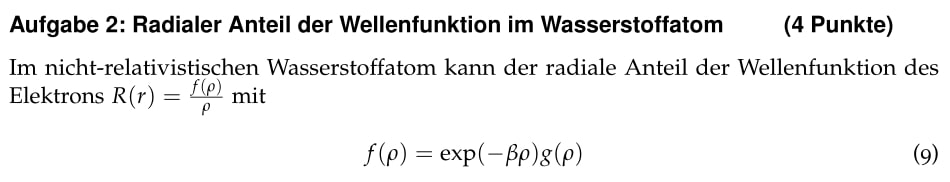
\includegraphics[width=\textwidth]{images/Aufgabe2a.jpg}
        \label{fig:3}
    \end{figure}

    \begin{figure}[H]
        \centering
        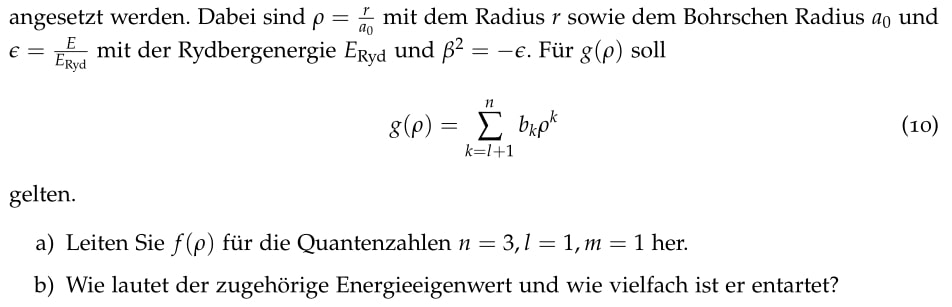
\includegraphics[width=\textwidth]{images/Aufgabe2b.jpg}
        \label{fig:4}
    \end{figure}

    \subsection{a)}

    \begin{align*}
        n &= 3,\;l = m = 1\\
        \\
        \Psi(r,\theta,\varphi) &= R(r)Y(\theta,\varphi)\\
        &= \frac{f(\rho)}{\rho} \sqrt{\frac{2l+1}{4\pi} \frac{(l-m)!}{(l+m)!}} P_l^m(\cos(\theta)) e^{im\varphi}
        \intertext{
            \flushleft{Mit\;}\justifying $P_1^1(\cos(\theta)) = -\sin(\theta)$ folgt:
        }
        &= \frac{f(\rho)}{\rho} \sqrt{\frac{3}{4\pi} \frac{1}{2}} (-\sin(\theta)) e^{i\varphi}
        \intertext{
            \flushleft{Das\;}\justifying $g(\rho)$ des Radialteils ist für $n=3$ und $l=1$ gleich $6\rho^2-\rho^3$. Daraus folgt für $f(\rho)$:
        }
        f(\rho) &= e^{-\beta\rho} 6\rho^2-\rho^3
        \intertext{
            \flushleft{Eingesetzt\;}\justifying ergibt sich für $\Psi$:
        }
        \Psi(r,\theta,\varphi) &= e^{-\beta\rho} \left( 6\rho-\rho^2 \right) \sqrt{\frac{3}{8\pi}} (-\sin(\theta)) e^{i\varphi}
    \end{align*}

    \subsection{b)}

    \flushleft{Der\;}\justifying Energieeigenwert lautet
    \begin{align*}
        E &= -E_{Ryd}\frac{1}{n^2} = -E_{Ryd}\frac{1}{9}
        \intertext{
            \flushleft{Für\;}\justifying die Quantenzahl $n=3$ ist die Energie $n^2$-fach, bzw. 9-fach entartet.
        }
    \end{align*}

\section{Aufgabe 3}

    \begin{figure}[H]
        \centering
        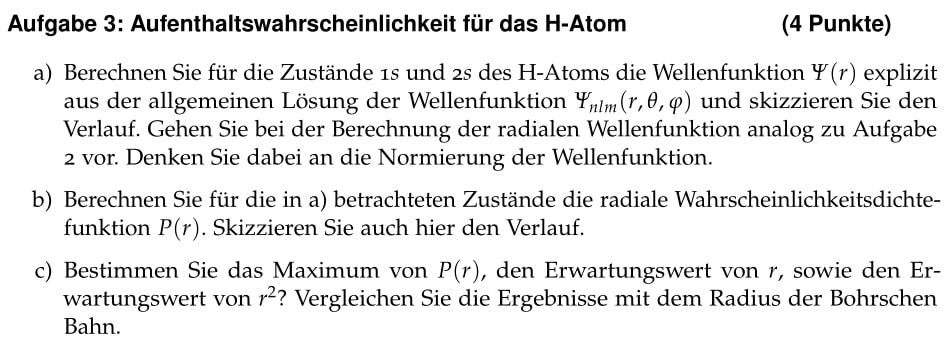
\includegraphics[width=\textwidth]{images/Aufgabe3.jpg}
        \label{fig:5}
    \end{figure}

    \subsection{a)}

    \flushleft{s1:\;}\justifying $n=1, l=m=0$
    \begin{align*}
        \Psi(r,\theta,\varphi) &= \frac{f(\rho)}{\rho} \sqrt{\frac{2l+1}{4\pi} \frac{(l-m)!}{(l+m)!}} P_l^m(\cos(\theta)) e^{im\varphi}
        \intertext{
            \flushleft{Für\;}\justifying $n=1,l=m=0$ ergibt sich für $P_0^0(\cos(\theta)) = 1$. Der Radialteil ist für $n=1$ und $l=0$ gleich $\rho$.
            Daraus folgt für $\Psi$:
        }
        &= e^{-\beta\rho} \sqrt{\frac{1}{4\pi} \frac{1}{1}} \cdot 1 \cdot e^0 = e^{-\beta\rho} \sqrt{\frac{1}{4\pi}}
        \intertext{
            \flushleft{s2:\;}\justifying $n=2, l=m=0$
        }
        g(\rho) &= e^{-\beta\rho} \frac{\rho-\frac{\rho^2}{2}}{\rho} = e^{-\beta\rho} \left(1-\frac{\rho}{2}\right)\\
        \Psi(r,\theta,\varphi) &= e^{-\beta\rho} \left(1-\frac{\rho}{2}\right) \sqrt{\frac{1}{4\pi}}
    \end{align*}

    \begin{figure}[H]
        \centering
        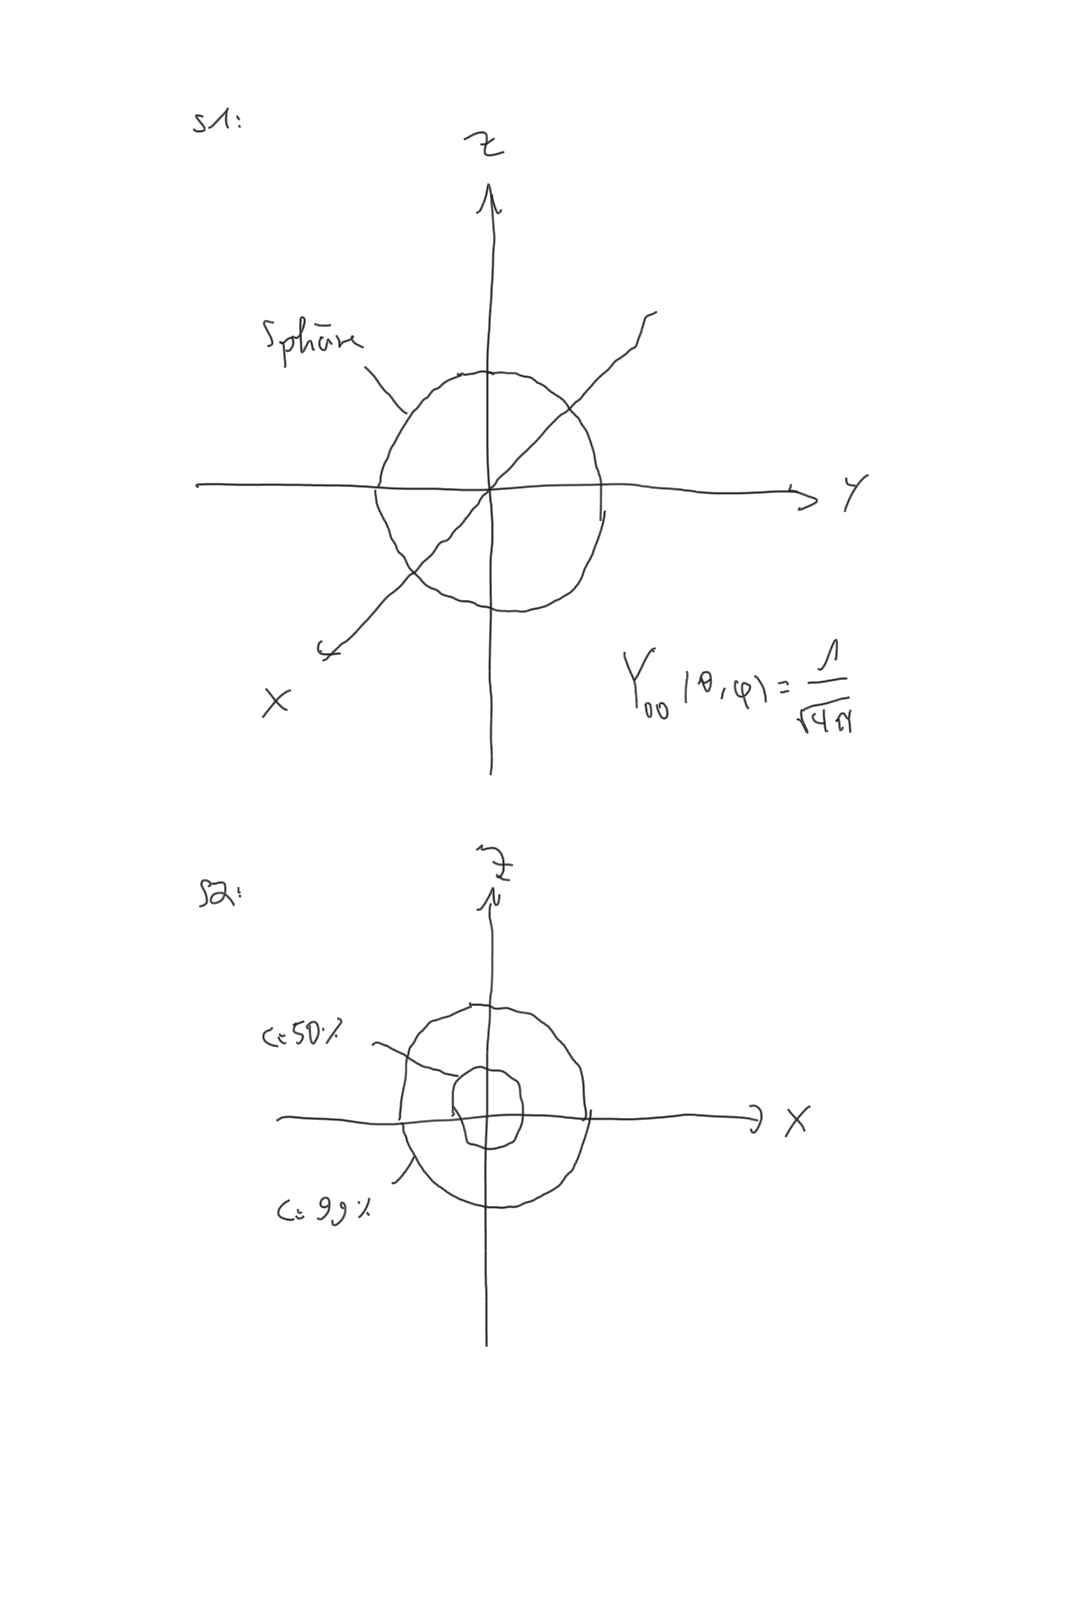
\includegraphics[width=\textwidth]{images/Skizze3a.jpg}
        \label{fig:6}
    \end{figure}

    \subsection{b)}

    \begin{align*}
        s1: P(r)\mathrm{d}r &= \int_{0}^{2\pi} \int_{0}^{\pi} \abs{\Psi(r,\theta,\varphi)}^2 r^2 \sin(\theta)\, \mathrm{d}r\, \mathrm{d}\theta\, \mathrm{d}\varphi\\
        &= \abs{R(r)}^2 r^2 \,\mathrm{d}r \int_{0}^{2\pi} \int_{0}^{\pi} \abs{Y(\theta,\varphi)}^2 \sin(\theta) \, \mathrm{d}\theta\, \mathrm{d}\varphi\\
        &= \abs{e^{-\beta\frac{r}{a_0}}}^2 r^2 \,\mathrm{d}r \int_{0}^{2\pi} \int_{0}^{\pi} \abs{\sqrt{\frac{1}{4\pi}}}^2 \sin(\theta) \, \mathrm{d}\theta\, \mathrm{d}\varphi\\
        &= \abs{e^{-\beta\frac{r}{a_0}}}^2 r^2 \,\mathrm{d}r \frac{1}{4\pi} \int_{0}^{2\pi} \left[-\cos(\theta)\right]_0^{\pi} \mathrm{d}\varphi\\
        &= \abs{e^{-\beta\frac{r}{a_0}}}^2 r^2 \,\mathrm{d}r \frac{1}{4\pi} 2\pi (1-(-1))\\
        &= e^{-2\beta\frac{r}{a_0}} r^2 \mathrm{d}r\\
        s2: P(r)\mathrm{d}r &= \int_{0}^{2\pi} \int_{0}^{\pi} \abs{\Psi(r,\theta,\varphi)}^2 r^2 \sin(\theta)\, \mathrm{d}r\, \mathrm{d}\theta\, \mathrm{d}\varphi\\
        &= \abs{R(r)}^2 r^2 \,\mathrm{d}r \int_{0}^{2\pi} \int_{0}^{\pi} \abs{Y(\theta,\varphi)}^2 \sin(\theta) \, \mathrm{d}\theta\, \mathrm{d}\varphi\\
        &= \abs{e^{-\beta\frac{r}{a_0}}\left( 1-\frac{r}{2 a_0} \right)}^2 r^2 \,\mathrm{d}r \int_{0}^{2\pi} \int_{0}^{\pi} \abs{\sqrt{\frac{1}{4\pi}}}^2 \sin(\theta) \, \mathrm{d}\theta\, \mathrm{d}\varphi\\
        &= \abs{e^{-\beta\frac{r}{a_0}}\left( 1-\frac{r}{2 a_0} \right)}^2 r^2 \,\mathrm{d}r \frac{1}{4\pi} \int_{0}^{2\pi} \left[-\cos(\theta)\right]_0^{\pi} \mathrm{d}\varphi\\
        &= \abs{e^{-\beta\frac{r}{a_0}}\left( 1-\frac{r}{2 a_0} \right)}^2 r^2 \,\mathrm{d}r \frac{1}{4\pi} 2\pi (1-(-1))\\
        &= e^{-2\beta\frac{r}{a_0}}\left( 1-\frac{r}{a_0} +\frac{r^2}{4 a_0^2} \right) r^2 \mathrm{d}r
    \end{align*}

    \begin{figure}[H]
        \centering
        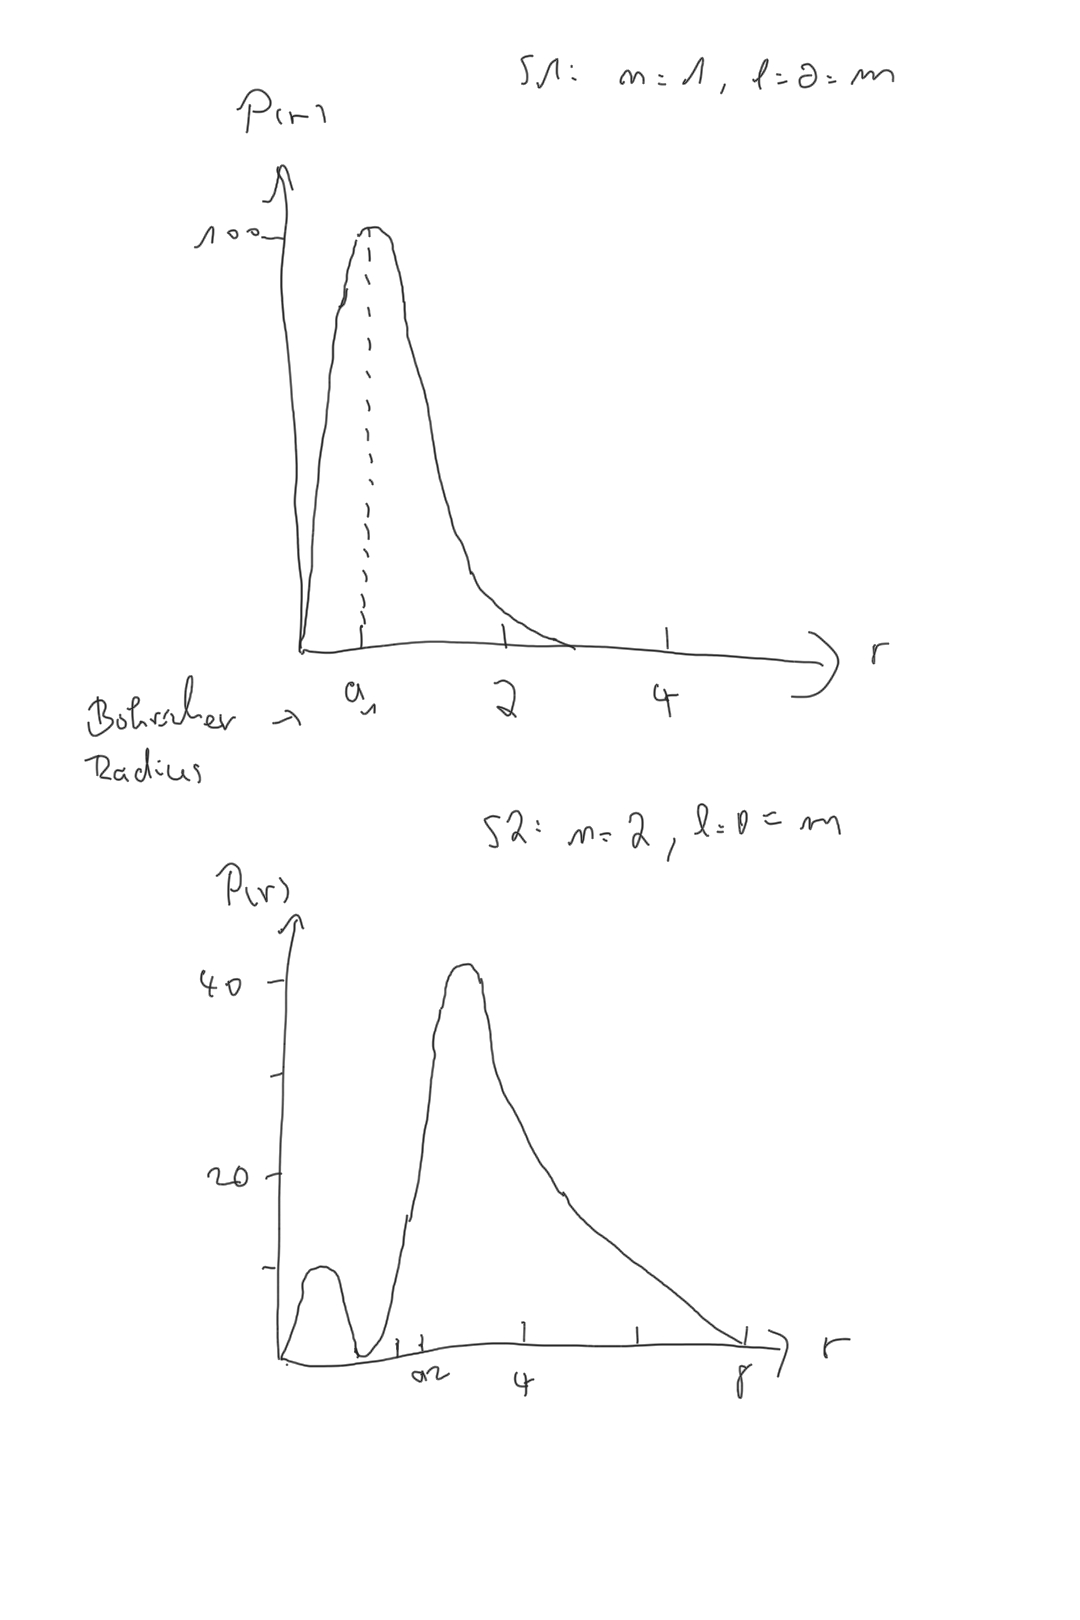
\includegraphics[width=\textwidth]{images/Skizze3b.jpg}
        \label{fig:7}
    \end{figure}

    \subsection{c)}

\section{Aufgabe 4}

    \begin{figure}[H]
        \centering
        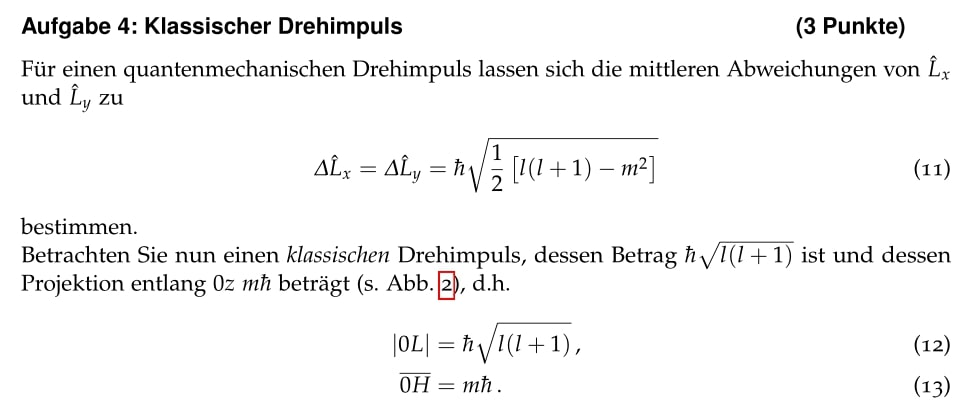
\includegraphics[width=\textwidth]{images/Aufgabe4a.jpg}
        \label{fig:8}
    \end{figure}

    \begin{figure}[H]
        \centering
        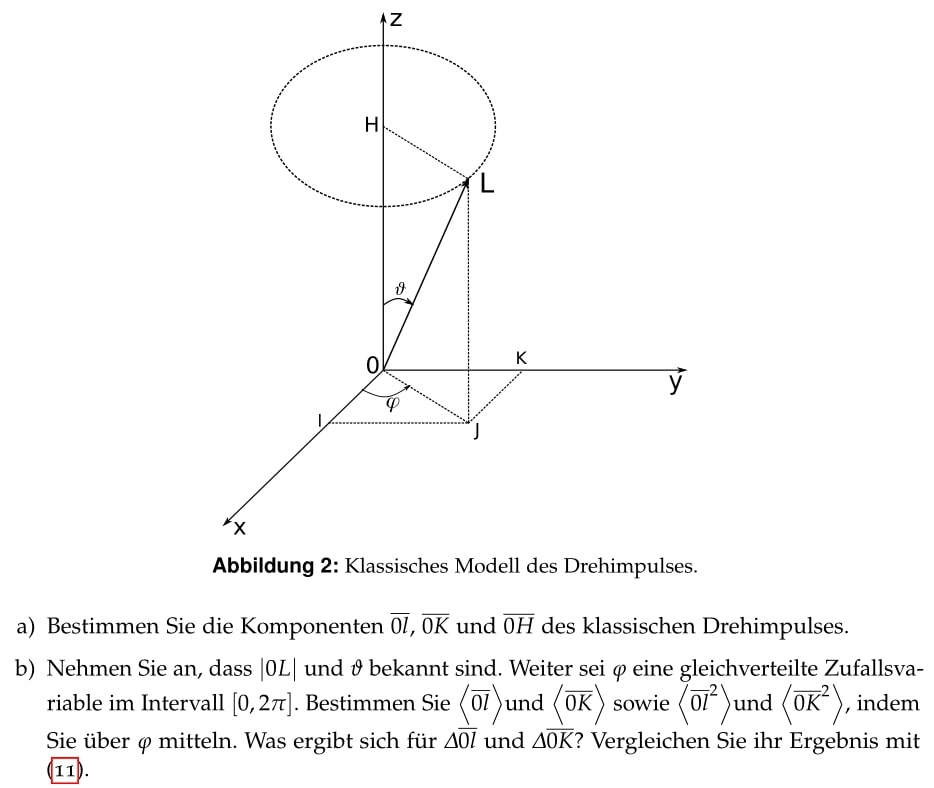
\includegraphics[width=\textwidth]{images/Aufgabe4b.jpg}
        \label{fig:9}
    \end{figure}

    \subsection{a)}

    \begin{align*}
        L_{x,y,z} &= \overline{0L} \Rightarrow \abs{0L} = \hbar\sqrt{l(l+1)}\\
        L_{x,y} &= \overline{0j} = \overline{0L} \cdot \sin(\theta) = \hbar\sqrt{l(l+1)}\\
        \\
        L_x &= \abs{0l} = \abs{0j} \cos(\varphi) = \abs{0L}\cos(\varphi)\sin(\theta)\\
        L_y &= \abs{0K} = \abs{0j} \sin(\varphi) = \abs{0L}\sin(\varphi)\sin(\theta)\\
        L_z &= \abs{0H} = \hbar m\\
        \vec{L} &= \begin{pmatrix}
            \abs{0L}\cos(\varphi)\sin(\theta)\\
            \abs{0L}\sin(\varphi)\sin(\theta)\\
            \hbar m
        \end{pmatrix}
    \end{align*}

    \subsection{b)}

    \begin{align*}
        \langle \abs{0l} \rangle &=  \langle L_x \rangle = \frac{1}{2\pi} \int_{0}^{2\pi} \abs{0L} \cos(\varphi) \sin(\theta) \,\mathrm{d}\varphi\\
        &= \frac{1}{2\pi} \abs{0L}\sin(\theta) \int_{0}^{2\pi} \cos(\varphi) \,\mathrm{d}\varphi\\
        &= 0\\
        \\
        \langle \abs{0K} \rangle &=  \langle L_y \rangle = \frac{1}{2\pi} \int_{0}^{2\pi} \abs{0L} \sin(\varphi) \sin(\theta) \,\mathrm{d}\varphi\\
        &= \frac{1}{2\pi} \abs{0L}\sin(\theta) \int_{0}^{2\pi} \sin(\varphi) \,\mathrm{d}\varphi\\
        &= 0\\
        \langle \abs{0l}^2 \rangle &= \frac{1}{2\pi} \int_{0}^{2\pi} \abs{0L}^2 \cos^2(\varphi) \sin^2(\theta) \,\mathrm{d}\varphi\\
        &= \frac{1}{2} \abs{0L}^2 \sin^2(\theta)\\
        &= \frac{1}{2} \abs{0j}^2\\
        \langle \abs{0K}^2 \rangle &= \frac{1}{2\pi} \int_{0}^{2\pi} \abs{0L}^2 \sin^2(\varphi) \sin^2(\theta) \,\mathrm{d}\varphi\\
        &= \frac{1}{2} \abs{0L}^2 \sin^2(\theta)\\
        &= \frac{1}{2} \abs{0j}^2\\
        \\
        \Rightarrow L_x &= L_y\\
        \Rightarrow \Delta L_x &= \Delta L_y = \sqrt{\langle \abs{0l}^2 \rangle - \langle \abs{0l} \rangle^2} = \sqrt{\langle \abs{0l}^2 \rangle} = \sqrt{\frac{1}{2} \abs{0j}^2} \\
        \abs{0L}^2 &= \abs{0H}^2 + \abs{0j}^2\\
        \Rightarrow \abs{0j} &= \sqrt{\abs{0L}^2-\abs{0H}^2}\\
        &= \sqrt{\frac{1}{2} \left( \hbar^2 l (l+1) -\hbar^2 m^2 \right)}\\
        &= \hbar \sqrt{\frac{1}{2} l(l+1) - m^2}
    \end{align*}









\end{document}